%%%% Paramétrage du TD %%%%
\def\xxactivite{\ifcolle Colle \else TD 1 \fi  \ifprof -- Corrigé \else \fi} % \normalsize \vspace{-.4cm}
\def\xxauteur{\textsl{Xavier Pessoles}}

\def\xxnumchapitre{Chapitre 4 \vspace{.2cm}}
\def\xxchapitre{\hspace{.12cm} Méthodologie : détermination des équations de mouvement}
\def\xxpartie{Modéliser le comportement des systèmes mécaniques dans le but d'établir une loi de comportement ou de déterminer des actions mécaniques en utilisant le PFD}



%\def\xxauteur{\textsl{Frédéric Sollner}}
%
% \ifnormal $\star$ \else \fi \iftdifficile $\star\star\star$ \else \fi
%\def\xxtitreexo{ }
%


\def\xxtitreexo{Dynamique du véhicule -- Segway de première génération\ifnormal $\star$ \else \fi \ifdifficile $\star\star$ \else \fi \iftdifficile $\star\star\star$ \else \fi }

\def\xxsourceexo{\hspace{.2cm} \footnotesize{Frédéric SOLLNER -- Lycée Mermoz -- Montpellier}}


\def\xxcompetences{%
\vspace{-.5cm}
\textsl{%
\textbf{Savoirs et compétences :}
\begin{itemize}[label=\ding{112},font=\color{ocre}] 
%\item \textit{Mod2.C16} : torseur cinétique
%\item \textit{Mod2.C17} : torseur dynamique
%\item \textit{Mod2.C17.SF1} : déterminer le torseur dynamique d’un solide, ou d’un ensemble de solides, par rapport à un autre solide
%\item \textit{Mod2.C15} : matrice d'inertie
\item \textit{Res1.C2} : principe fondamental de la dynamique
\item \textit{Res1.C1.SF1} : proposer une démarche permettant la détermination de la loi de mouvement
%\item \textit{Res1.C2.SF1} : proposer une méthode permettant la détermination d’une inconnue de liaison
\end{itemize}
}}
\def\xxfigures{
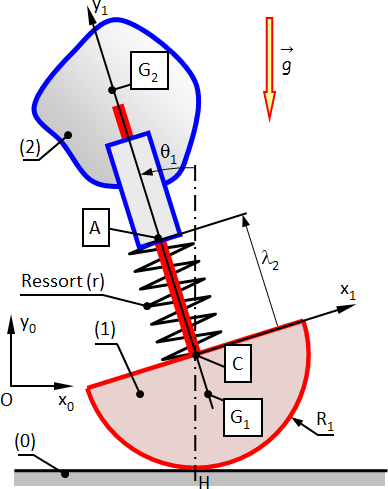
\includegraphics[width=.3\textwidth]{fig_01}
}%figues de la page de garde


\iflivret
\pagestyle{empty}


%%%%%%%% PAGE DE GARDE COURS
\ifcours
% ==== BANDEAU DES TITRES ==== 
\begin{tikzpicture}[remember picture,overlay]
\node at (current page.north west)
{\begin{tikzpicture}[remember picture,overlay]
\node[anchor=north west,inner sep=0pt] at (0,0) {\includegraphics[width=\paperwidth]{\thechapterimage}};
\draw[anchor=west] (-2cm,-8cm) node [line width=2pt,rounded corners=15pt,draw=ocre,fill=white,fill opacity=0.6,inner sep=40pt]{\strut\makebox[22cm]{}};
\draw[anchor=west] (1cm,-8cm) node {\huge\sffamily\bfseries\color{black} %
\begin{minipage}{1cm}
\rotatebox{90}{\LARGE\sffamily\textsc{\color{ocre}\textbf{\xxnumpartie}}}
\end{minipage} \hfill
\begin{minipage}[c]{14cm}
\begin{titrepartie}
\begin{flushright}
\renewcommand{\baselinestretch}{1.1} 
\Large\sffamily\textsc{\textbf{\xxpartie}}
\renewcommand{\baselinestretch}{1} 
\end{flushright}
\end{titrepartie}
\end{minipage} \hfill
\begin{minipage}[c]{3.5cm}
{\large\sffamily\textsc{\textbf{\color{ocre} \discipline}}}
\end{minipage} 
 };
\end{tikzpicture}};
\end{tikzpicture}
% ==== FIN BANDEAU DES TITRES ==== 


% ==== ONGLET 
\begin{tikzpicture}[overlay]
\node[shape=rectangle, 
      rounded corners = .25 cm,
	  draw= ocre,
	  line width=2pt, 
	  fill = ocre!10,
	  minimum width  = 2.5cm,
	  minimum height = 3cm,] at (18.3cm,0) {};
\node at (17.7cm,0) {\rotatebox{90}{\textbf{\Large\color{ocre}{\classe}}}};
%{};
\end{tikzpicture}
% ==== FIN ONGLET 


\vspace{3.5cm}

\begin{tikzpicture}[remember picture,overlay]
\draw[anchor=west] (-2cm,-6cm) node {\huge\sffamily\bfseries\color{black} %
\begin{minipage}{2cm}
\begin{center}
\LARGE\sffamily\textsc{\color{ocre}\textbf{\xxactivite}}
\end{center}
\end{minipage} \hfill
\begin{minipage}[c]{15cm}
\begin{titrechapitre}
\renewcommand{\baselinestretch}{1.1} 
\Large\sffamily\textsc{\textbf{\xxnumchapitre}}

\Large\sffamily\textsc{\textbf{\xxchapitre}}
\vspace{.5cm}

\renewcommand{\baselinestretch}{1} 
\normalsize\normalfont
\xxcompetences
\end{titrechapitre}
\end{minipage}  };
\end{tikzpicture}
\vfill

\begin{flushright}
\begin{minipage}[c]{.3\linewidth}
\begin{center}
\xxfigures
\end{center}
\end{minipage}\hfill
\begin{minipage}[c]{.6\linewidth}
\startcontents
%\printcontents{}{1}{}
\printcontents{}{1}{}
\end{minipage}
\end{flushright}

\begin{tikzpicture}[remember picture,overlay]
\draw[anchor=west] (4.5cm,-.7cm) node {
\begin{minipage}[c]{.2\linewidth}
\begin{flushright}

\includegraphics[width=2cm]{logoCC}
\end{flushright}
\end{minipage}
\begin{minipage}[c]{.2\linewidth}
\textsl{\xxauteur} \\
\textsl{\classe}
\end{minipage}
 };
\end{tikzpicture}

\newpage
\pagestyle{fancy}

%\newpage
%\pagestyle{fancy}

\else
\fi
%% FIN PAGE DE GARDE DES COURS

%%%%%%%% PAGE DE GARDE TD
\iftd
%\begin{tikzpicture}[remember picture,overlay]
%\node at (current page.north west)
%{\begin{tikzpicture}[remember picture,overlay]
%\draw[anchor=west] (-2cm,-3.25cm) node [line width=2pt,rounded corners=15pt,draw=ocre,fill=white,fill opacity=0.6,inner sep=40pt]{\strut\makebox[22cm]{}};
%\draw[anchor=west] (1cm,-3.25cm) node {\huge\sffamily\bfseries\color{black} %
%\begin{minipage}{1cm}
%\rotatebox{90}{\LARGE\sffamily\textsc{\color{ocre}\textbf{\xxnumpartie}}}
%\end{minipage} \hfill
%\begin{minipage}[c]{13.5cm}
%\begin{titrepartie}
%\begin{flushright}
%\renewcommand{\baselinestretch}{1.1} 
%\Large\sffamily\textsc{\textbf{\xxpartie}}
%\renewcommand{\baselinestretch}{1} 
%\end{flushright}
%\end{titrepartie}
%\end{minipage} \hfill
%\begin{minipage}[c]{3.5cm}
%{\large\sffamily\textsc{\textbf{\color{ocre} \discipline}}}
%\end{minipage} 
% };
%\end{tikzpicture}};
%\end{tikzpicture}

%%%%%%%%%% PAGE DE GARDE TD %%%%%%%%%%%%%%%
%\begin{tikzpicture}[overlay]
%\node[shape=rectangle, 
%      rounded corners = .25 cm,
%	  draw= ocre,
%	  line width=2pt, 
%	  fill = ocre!10,
%	  minimum width  = 2.5cm,
%	  minimum height = 2.5cm,] at (18.5cm,0) {};
%\node at (17.7cm,0) {\rotatebox{90}{\textbf{\Large\color{ocre}{\classe}}}};
%%{};
%\end{tikzpicture}

% PARTIE ET CHAPITRE
%\begin{tikzpicture}[remember picture,overlay]
%\draw[anchor=west] (-1cm,-2.1cm) node {\large\sffamily\bfseries\color{black} %
%\begin{minipage}[c]{15cm}
%\begin{flushleft}
%\xxnumchapitre \\
%\xxchapitre
%\end{flushleft}
%\end{minipage}  };
%\end{tikzpicture}

% BANDEAU EXO
\iflivret % SI LIVRET
\begin{tikzpicture}[remember picture,overlay]
\draw[anchor=west] (-2cm,-3.3cm) node {\huge\sffamily\bfseries\color{black} %
\begin{minipage}{5cm}
\begin{center}
\LARGE\sffamily\color{ocre}\textbf{\textsc{\xxactivite}}

\begin{center}
\xxfigures
\end{center}

\end{center}
\end{minipage} \hfill
\begin{minipage}[c]{12cm}
\begin{titrechapitre}
\renewcommand{\baselinestretch}{1.1} 
\large\sffamily\textbf{\textsc{\xxtitreexo}}

\small\sffamily{\textbf{\textit{\color{black!70}\xxsourceexo}}}
\vspace{.5cm}

\renewcommand{\baselinestretch}{1} 
\normalsize\normalfont
\xxcompetences
\end{titrechapitre}
\end{minipage}};
\end{tikzpicture}
\else % ELSE NOT LIVRET
\begin{tikzpicture}[remember picture,overlay]
\draw[anchor=west] (-2cm,-4.5cm) node {\huge\sffamily\bfseries\color{black} %
\begin{minipage}{5cm}
\begin{center}
\LARGE\sffamily\color{ocre}\textbf{\textsc{\xxactivite}}

\begin{center}
\xxfigures
\end{center}

\end{center}
\end{minipage} \hfill
\begin{minipage}[c]{12cm}
\begin{titrechapitre}
\renewcommand{\baselinestretch}{1.1} 
\large\sffamily\textbf{\textsc{\xxtitreexo}}

\small\sffamily{\textbf{\textit{\color{black!70}\xxsourceexo}}}
\vspace{.5cm}

\renewcommand{\baselinestretch}{1} 
\normalsize\normalfont
\xxcompetences
\end{titrechapitre}
\end{minipage}};
\end{tikzpicture}

\fi

\else   % FIN IF TD
\fi


%%%%%%%% PAGE DE GARDE FICHE
\iffiche
\begin{tikzpicture}[remember picture,overlay]
\node at (current page.north west)
{\begin{tikzpicture}[remember picture,overlay]
\draw[anchor=west] (-2cm,-2.25cm) node [line width=2pt,rounded corners=15pt,draw=ocre,fill=white,fill opacity=0.6,inner sep=40pt]{\strut\makebox[22cm]{}};
\draw[anchor=west] (1cm,-2.25cm) node {\huge\sffamily\bfseries\color{black} %
\begin{minipage}{1cm}
\rotatebox{90}{\LARGE\sffamily\textsc{\color{ocre}\textbf{\xxnumpartie}}}
\end{minipage} \hfill
\begin{minipage}[c]{14cm}
\begin{titrepartie}
\begin{flushright}
\renewcommand{\baselinestretch}{1.1} 
\large\sffamily\textsc{\textbf{\xxpartie} \\} 

\vspace{.2cm}

\normalsize\sffamily\textsc{\textbf{\xxnumchapitre -- \xxchapitre}}
\renewcommand{\baselinestretch}{1} 
\end{flushright}
\end{titrepartie}
\end{minipage} \hfill
\begin{minipage}[c]{3.5cm}
{\large\sffamily\textsc{\textbf{\color{ocre} \discipline}}}
\end{minipage} 
 };
\end{tikzpicture}};
\end{tikzpicture}

\iflivret
\begin{tikzpicture}[overlay]
\node[shape=rectangle, 
      rounded corners = .25 cm,
	  draw= ocre,
	  line width=2pt, 
	  fill = ocre!10,
	  minimum width  = 2.5cm,
	  minimum height = 2.5cm,] at (18.5cm,.5cm) {};
\node at (17.9cm,.5cm) {\rotatebox{90}{\textsf{\textbf{\large\color{ocre}{\classe}}}}};
%{};
\end{tikzpicture}
\else
\begin{tikzpicture}[overlay]
\node[shape=rectangle, 
      rounded corners = .25 cm,
	  draw= ocre,
	  line width=2pt, 
	  fill = ocre!10,
	  minimum width  = 2.5cm,
%	  minimum height = 2.5cm,] at (18.5cm,1.1cm) {};
	  minimum height = 2.5cm,] at (18.6cm,0.5cm) {};
\node at (18cm,0.5cm) {\rotatebox{90}{\textsf{\textbf{\large\color{ocre}{\classe}}}}};
%{};
\end{tikzpicture}

\fi

\else
\fi



\else
\pagestyle{empty}


%%%%%%%% PAGE DE GARDE COURS
\ifcours
% ==== BANDEAU DES TITRES ==== 
\begin{tikzpicture}[remember picture,overlay]
\node at (current page.north west)
{\begin{tikzpicture}[remember picture,overlay]
\node[anchor=north west,inner sep=0pt] at (0,0) {\includegraphics[width=\paperwidth]{\thechapterimage}};
\draw[anchor=west] (-2cm,-8cm) node [line width=2pt,rounded corners=15pt,draw=ocre,fill=white,fill opacity=0.6,inner sep=40pt]{\strut\makebox[22cm]{}};
\draw[anchor=west] (1cm,-8cm) node {\huge\sffamily\bfseries\color{black} %
\begin{minipage}{1cm}
\rotatebox{90}{\LARGE\sffamily\textsc{\color{ocre}\textbf{\xxnumpartie}}}
\end{minipage} \hfill
\begin{minipage}[c]{14cm}
\begin{titrepartie}
\begin{flushright}
\renewcommand{\baselinestretch}{1.1} 
\Large\sffamily\textsc{\textbf{\xxpartie}}
\renewcommand{\baselinestretch}{1} 
\end{flushright}
\end{titrepartie}
\end{minipage} \hfill
\begin{minipage}[c]{3.5cm}
{\large\sffamily\textsc{\textbf{\color{ocre} \discipline}}}
\end{minipage} 
 };
\end{tikzpicture}};
\end{tikzpicture}
% ==== FIN BANDEAU DES TITRES ==== 


% ==== ONGLET 
\begin{tikzpicture}[overlay]
\node[shape=rectangle, 
      rounded corners = .25 cm,
	  draw= ocre,
	  line width=2pt, 
	  fill = ocre!10,
	  minimum width  = 2.5cm,
	  minimum height = 3cm,] at (18.3cm,0) {};
\node at (17.7cm,0) {\rotatebox{90}{\textbf{\Large\color{ocre}{\classe}}}};
%{};
\end{tikzpicture}
% ==== FIN ONGLET 


\vspace{3.5cm}

\begin{tikzpicture}[remember picture,overlay]
\draw[anchor=west] (-2cm,-6cm) node {\huge\sffamily\bfseries\color{black} %
\begin{minipage}{2cm}
\begin{center}
\LARGE\sffamily\textsc{\color{ocre}\textbf{\xxactivite}}
\end{center}
\end{minipage} \hfill
\begin{minipage}[c]{15cm}
\begin{titrechapitre}
\renewcommand{\baselinestretch}{1.1} 
\Large\sffamily\textsc{\textbf{\xxnumchapitre}}

\Large\sffamily\textsc{\textbf{\xxchapitre}}
\vspace{.5cm}

\renewcommand{\baselinestretch}{1} 
\normalsize\normalfont
\xxcompetences
\end{titrechapitre}
\end{minipage}  };
\end{tikzpicture}
\vfill

\begin{flushright}
\begin{minipage}[c]{.3\linewidth}
\begin{center}
\xxfigures
\end{center}
\end{minipage}\hfill
\begin{minipage}[c]{.6\linewidth}
\startcontents
%\printcontents{}{1}{}
\printcontents{}{1}{}
\end{minipage}
\end{flushright}

\begin{tikzpicture}[remember picture,overlay]
\draw[anchor=west] (4.5cm,-.7cm) node {
\begin{minipage}[c]{.2\linewidth}
\begin{flushright}

\includegraphics[width=2cm]{logoCC}
\end{flushright}
\end{minipage}
\begin{minipage}[c]{.2\linewidth}
\textsl{\xxauteur} \\
\textsl{\classe}
\end{minipage}
 };
\end{tikzpicture}

\newpage
\pagestyle{fancy}

%\newpage
%\pagestyle{fancy}

\else
\fi
%% FIN PAGE DE GARDE DES COURS

%%%%%%%% PAGE DE GARDE TD
\iftd
%\begin{tikzpicture}[remember picture,overlay]
%\node at (current page.north west)
%{\begin{tikzpicture}[remember picture,overlay]
%\draw[anchor=west] (-2cm,-3.25cm) node [line width=2pt,rounded corners=15pt,draw=ocre,fill=white,fill opacity=0.6,inner sep=40pt]{\strut\makebox[22cm]{}};
%\draw[anchor=west] (1cm,-3.25cm) node {\huge\sffamily\bfseries\color{black} %
%\begin{minipage}{1cm}
%\rotatebox{90}{\LARGE\sffamily\textsc{\color{ocre}\textbf{\xxnumpartie}}}
%\end{minipage} \hfill
%\begin{minipage}[c]{13.5cm}
%\begin{titrepartie}
%\begin{flushright}
%\renewcommand{\baselinestretch}{1.1} 
%\Large\sffamily\textsc{\textbf{\xxpartie}}
%\renewcommand{\baselinestretch}{1} 
%\end{flushright}
%\end{titrepartie}
%\end{minipage} \hfill
%\begin{minipage}[c]{3.5cm}
%{\large\sffamily\textsc{\textbf{\color{ocre} \discipline}}}
%\end{minipage} 
% };
%\end{tikzpicture}};
%\end{tikzpicture}

%%%%%%%%%% PAGE DE GARDE TD %%%%%%%%%%%%%%%
%\begin{tikzpicture}[overlay]
%\node[shape=rectangle, 
%      rounded corners = .25 cm,
%	  draw= ocre,
%	  line width=2pt, 
%	  fill = ocre!10,
%	  minimum width  = 2.5cm,
%	  minimum height = 2.5cm,] at (18.5cm,0) {};
%\node at (17.7cm,0) {\rotatebox{90}{\textbf{\Large\color{ocre}{\classe}}}};
%%{};
%\end{tikzpicture}

% PARTIE ET CHAPITRE
%\begin{tikzpicture}[remember picture,overlay]
%\draw[anchor=west] (-1cm,-2.1cm) node {\large\sffamily\bfseries\color{black} %
%\begin{minipage}[c]{15cm}
%\begin{flushleft}
%\xxnumchapitre \\
%\xxchapitre
%\end{flushleft}
%\end{minipage}  };
%\end{tikzpicture}

% BANDEAU EXO
\iflivret % SI LIVRET
\begin{tikzpicture}[remember picture,overlay]
\draw[anchor=west] (-2cm,-3.3cm) node {\huge\sffamily\bfseries\color{black} %
\begin{minipage}{5cm}
\begin{center}
\LARGE\sffamily\color{ocre}\textbf{\textsc{\xxactivite}}

\begin{center}
\xxfigures
\end{center}

\end{center}
\end{minipage} \hfill
\begin{minipage}[c]{12cm}
\begin{titrechapitre}
\renewcommand{\baselinestretch}{1.1} 
\large\sffamily\textbf{\textsc{\xxtitreexo}}

\small\sffamily{\textbf{\textit{\color{black!70}\xxsourceexo}}}
\vspace{.5cm}

\renewcommand{\baselinestretch}{1} 
\normalsize\normalfont
\xxcompetences
\end{titrechapitre}
\end{minipage}};
\end{tikzpicture}
\else % ELSE NOT LIVRET
\begin{tikzpicture}[remember picture,overlay]
\draw[anchor=west] (-2cm,-4.5cm) node {\huge\sffamily\bfseries\color{black} %
\begin{minipage}{5cm}
\begin{center}
\LARGE\sffamily\color{ocre}\textbf{\textsc{\xxactivite}}

\begin{center}
\xxfigures
\end{center}

\end{center}
\end{minipage} \hfill
\begin{minipage}[c]{12cm}
\begin{titrechapitre}
\renewcommand{\baselinestretch}{1.1} 
\large\sffamily\textbf{\textsc{\xxtitreexo}}

\small\sffamily{\textbf{\textit{\color{black!70}\xxsourceexo}}}
\vspace{.5cm}

\renewcommand{\baselinestretch}{1} 
\normalsize\normalfont
\xxcompetences
\end{titrechapitre}
\end{minipage}};
\end{tikzpicture}

\fi

\else   % FIN IF TD
\fi


%%%%%%%% PAGE DE GARDE FICHE
\iffiche
\begin{tikzpicture}[remember picture,overlay]
\node at (current page.north west)
{\begin{tikzpicture}[remember picture,overlay]
\draw[anchor=west] (-2cm,-2.25cm) node [line width=2pt,rounded corners=15pt,draw=ocre,fill=white,fill opacity=0.6,inner sep=40pt]{\strut\makebox[22cm]{}};
\draw[anchor=west] (1cm,-2.25cm) node {\huge\sffamily\bfseries\color{black} %
\begin{minipage}{1cm}
\rotatebox{90}{\LARGE\sffamily\textsc{\color{ocre}\textbf{\xxnumpartie}}}
\end{minipage} \hfill
\begin{minipage}[c]{14cm}
\begin{titrepartie}
\begin{flushright}
\renewcommand{\baselinestretch}{1.1} 
\large\sffamily\textsc{\textbf{\xxpartie} \\} 

\vspace{.2cm}

\normalsize\sffamily\textsc{\textbf{\xxnumchapitre -- \xxchapitre}}
\renewcommand{\baselinestretch}{1} 
\end{flushright}
\end{titrepartie}
\end{minipage} \hfill
\begin{minipage}[c]{3.5cm}
{\large\sffamily\textsc{\textbf{\color{ocre} \discipline}}}
\end{minipage} 
 };
\end{tikzpicture}};
\end{tikzpicture}

\iflivret
\begin{tikzpicture}[overlay]
\node[shape=rectangle, 
      rounded corners = .25 cm,
	  draw= ocre,
	  line width=2pt, 
	  fill = ocre!10,
	  minimum width  = 2.5cm,
	  minimum height = 2.5cm,] at (18.5cm,.5cm) {};
\node at (17.9cm,.5cm) {\rotatebox{90}{\textsf{\textbf{\large\color{ocre}{\classe}}}}};
%{};
\end{tikzpicture}
\else
\begin{tikzpicture}[overlay]
\node[shape=rectangle, 
      rounded corners = .25 cm,
	  draw= ocre,
	  line width=2pt, 
	  fill = ocre!10,
	  minimum width  = 2.5cm,
%	  minimum height = 2.5cm,] at (18.5cm,1.1cm) {};
	  minimum height = 2.5cm,] at (18.6cm,0.5cm) {};
\node at (18cm,0.5cm) {\rotatebox{90}{\textsf{\textbf{\large\color{ocre}{\classe}}}}};
%{};
\end{tikzpicture}

\fi

\else
\fi



\fi
\setlength{\columnseprule}{.1pt}

\pagestyle{fancy}
\thispagestyle{plain}

\ifprof
\vspace{4.8cm}
\else
\vspace{4.8cm}
\fi

\def\columnseprulecolor{\color{ocre}}
\setlength{\columnseprule}{0.4pt} 




\ifprof
%\begin{multicols}{2}
\else
\begin{multicols}{2}
\fi

\section*{Présentation}
\ifprof
\else

Le support de l’étude est le véhicule auto balancé Segway®. Il s’agit d’un moyen de transport motorisé qui permet de se déplacer en ville. En termes de prestations, il est moins rapide qu’une voiture ou qu’un scooter, mais plus maniable, plus écologique, moins encombrant et nettement plus moderne.

	La première génération de Segway avait un guidon fixe et une poignée de direction). Cette technologie provoquait un effet de roulis qui pouvait conduire à un renversement. Dans cet exercice, nous nous proposons d’étudier le dérapage et le renversement d’un Segway de première génération.
	
	La seconde génération de Segway a vu apparaître une technologie appelée LeanSteer avec guidon inclinable qui permet de faire tourner le Segway lorsque l'utilisateur penche son corps sur le côté (non étudié dans cet exercice).

\begin{center}
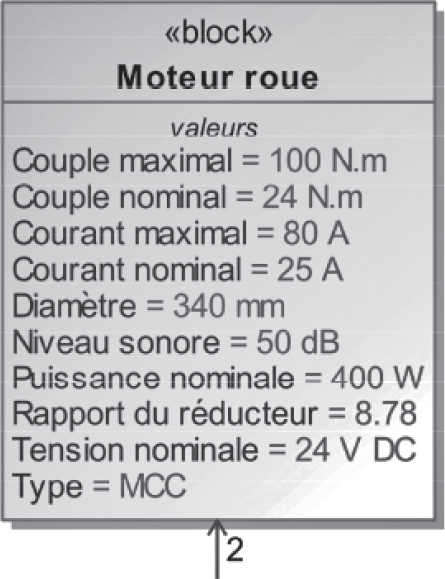
\includegraphics[width=\linewidth]{fig_02}
%\textit{Modèle volumique 3D}
\end{center}


On donne les caractéristiques géométriques et cinématiques suivantes :
\begin{itemize}
\item la route \textbf{(0)} est munie du repère $\rep{0}=\repere{O}{x_0}{y_0}{z_0}$. Ce référentiel associé est supposé galiléen.
\item la plate-forme \textbf{(1)} a pour centre de gravité $C$. Le conducteur \textbf{(2)} a pour centre de gravité $G$. Les roues 3 et 4,de masse et inertie négligeable, sont liées à 1 par des liaisons pivots d'axe $\axe{C}{y_1}$. L’ensemble 
$E=1\cup 2$ forme le système matériel indéformable $E$ de centre de gravité $G_E$ et de masse $m_E$. Il est animée d'un mouvement de rotation par rapport au sol dont le centre instantané de rotation est $O$. Le rayon de courbure de la trajectoire du point $G_E$ dans $\rep{0}$ est $\rep{C}$. Le repère lié à 1 est $\rep{1}$  tel que $\vect{z_1}=\vect{z_0}=\vect{z_{01}}=$ et on note $\theta=\angl{x_0}{x_1}=\angl{y_0}{y_1}$. 
\end{itemize}


On donne $\vect{OG_E}=R_C\vect{y_1}+h\vect{z}_{01}$. L'opérateur d'inertie de $E$ en $G_E$ dans $\mathcal{B}_1=\base{x_1}{y_1}{z_1}$ est : 
$\inertie{G_E}{E}=\matinertie{A}{B}{C}{-D}{-E}{-F}{\mathcal{B}_1}$.

\begin{hypo}
\begin{itemize} 
\item Les contacts entre les roues 3 et 4 et la route 0 ont lieu en $A$ et $B$ définis par $\vect{G_EA}=-l\vect{y_1}-h\vect{z_0}$ et $\vect{G_EB}=l\vect{y_1}-h\vect{z_0}$, $l$ désignant la demi voie du véhicule. Les contacts sont modélisés par des liaisons sphère-plan de centres $A$ et $B$ et de normale $\vect{z_{01}}$. Le contact dans ces liaisons se fait avec un coefficient de frottement noté $f$ (on supposera pour simplifier que les coefficients de frottement et d'adhérence sont identiques). Les actions mécaniques de la route 0 sur les roues 3 et 4 sont modélisées par des glisseurs en $A$ et $B$ de résultantes $\vectf{0}{3}=-T_A\vect{y_1}+N_A\vect{z_1}$ et $\vectf{0}{4}=-T_B\vect{y_1}+N_B\vect{z_1}$.
\item On se place dans un cas où le rayon de courbure $R_C$ de la trajectoire du point $C$, ainsi que la vitesse de rotation $\dot{\theta}$ par rapport au référentiel $\rep{0}$ sont constants.
\item L'accélération de la pesanteur est $\vect{g}=-g\vect{z_0}$. Accélération de la pesanteur, $g=\SI{10}{ms^{-2}}$.
\item On néglige la masse et les l'inertie des roues. 
%\item On considère que le couple moteur est nul.
\end{itemize}
\end{hypo}
On donne : 	
\begin{itemize}
\item coefficient d'adhérence pneu-route :  $f=1$;
\item masse de $E=1+2$:  $m_E=\SI{134}{kg}$;
\item demi largeur des voies :  $l=\SI{35}{cm}$,  $h=\SI{86}{cm}$.
\end{itemize}
\fi

\begin{obj}
L'objectif est de valider l'exigence 1 : permettre à l'utilisateur de se déplacer sur le sol.
\end{obj}

\subsection*{Étude du dérapage en virage du véhicule Segway}
\ifprof

\else
On donne ci-dessous un extrait du cahier des charges.

%\begin{obj} ~\\
\begin{center}
\begin{tabular}{|p{.7\linewidth}|p{.2\linewidth}|}
\hline 
Exigence & Niveau \\
\hline
id=<<1.1>> Glissement du véhicule pour une vitesse de $\SI{20}{km.h^{-1}}$ dans un virage de rayon de courbure \SI{10}{m} 
& Interdit \\
\hline
\end{tabular}
\end{center}
%\end{obj}

\fi

\subparagraph{}\textit{Exprimer la vitesse, notée  $\vect{V\left(G_E /\rep{0}\right)}$, du point $G_E$ dans son mouvement par rapport à $\rep{0}$ en fonction de $\dot{\theta}$ et $R_C$. Exprimer la vitesse linéaire du véhicule en fonction de $R_C$ et $\dot{\theta}$.}

\ifprof
\begin{corrige}
On a $\vect{V\left(G_E /\rep{0}\right)}=-R_C\dot{\theta}\vect{x_1}$. On a alors $V_L=R_C\dot{\theta}$. 
\end{corrige}
\else
\fi

\ifnormal
\subparagraph{}\textit{Exprimer l'accélération, notée  $\vect{\Gamma \left(G_E /\rep{0}\right)}$, du point $G_E$ dans son mouvement par rapport à $\rep{0}$ en fonction de $\dot{\theta}$ et $R_C$.}
\else
\fi


\ifprof
\begin{corrige}
$\vect{\Gamma \left(G_E /\rep{0}\right)}=\left[\dfrac{\dd \vect{V\left(G_E /\rep{0}\right)}}{\dd t}\right]_{\rep{0}}= 
-R_C\ddot{\theta}\vect{x_1}-R_C\dot{\theta}^2\vect{y_1}=-R_C\dot{\theta}^2\vect{y_1}$ ($\dot{\theta}$ est constant).
\end{corrige}
\else
\fi

\ifnormal
\subparagraph{}\textit{Exprimer les conditions d'adhérence liant $T_A$, $T_B$, $N_A$, $N_B$ et $f$ traduisant le non glissement du véhicule. En déduire une inéquation liant $T_A + T_B$ à $f$ et $N_A + N_B$.}
\else
\fi

\ifprof
\begin{corrige}
La direction des efforts normaux et tangentiels est donnée. En utilisant les lois de Coulomb, on a donc, $T_A\leq fN_A$ et $T_B\leq fN_B$. En sommant les inégalités, on a donc $T_A+T_B\leq f\left(N_A+N_B\right)$.
\end{corrige}
\else
\fi

\ifnormal
\subparagraph{}\textit{Isoler $E$ et les roues. Écrire le théorème de la résultante dynamique en projection sur $\vect{z_0}$.}% En déduire une inéquation liant $T_A + T_B$ à $f$, $m_E$ et $g$.}
\else
\fi
\ifprof
\begin{corrige}
$E$ étant un ensemble indéformable, on a : $\vectrd{E}{\rep{0}}=-m_E R_C\dot{\theta}^2\vect{y_1}$ (pas de projection sur $\vect{z_0}$. 
On isole $E$ et les roues  et on réalise le BAME : 
\begin{itemize}
\item pesanteur sur $E$;
\item action du sol sur les roues.
\end{itemize}

En appliquant le TRD en projection sur $\vect{z_{01}}$, on a donc :
$N_A+N_B-m_E g = 0$. 

%En conséquence, $T_A+T_B\leq fm_E g $.

\end{corrige}
\else
\fi

\ifnormal
\subparagraph{}\textit{Isoler $E$ et les roues. Écrire le théorème de la résultante dynamique en projection sur $\vect{y_1}$ . En déduire une inéquation donnant la vitesse limite $V_L$ de passage dans un virage qui ne provoque pas le dérapage.}
\else
\fi

\ifprof

\begin{corrige}
En appliquant le TRD en projection sur $\vect{y_{1}}$, on a : $-T_A-T_B = -m_E R_C\dot{\theta}^2$ $\Leftrightarrow T_A+T_B = m_E R_C\dot{\theta}^2$. En utilisant les résultats de la question précédente, $m_E R_C\dot{\theta}^2 \leq fm_E g $. En notant $V_L=R_C\dot{\theta}$ la vitesse limite avant dérapage, on a $ \dfrac{V_L^2}{R_C} \leq f  g $.
On a donc $V_L \leq \sqrt{R_Cfg}$.
\end{corrige}
\else
\fi

\ifnormal
\subparagraph{}\textit{Faire les applications numériques nécessaires et vérifier la conformité au cahier des charges.}
\else
\fi
\ifprof
\begin{corrige}
La vitesse limite est donc de \SI{10}{m.s^{-1}} soient \SI{36}{km.h^{-1}} ce qui satisfait le cahier des charges. 
\end{corrige}
\else
\fi

\iftdifficile
\subparagraph{}\textit{Exprimer la vitesse limite pour laquelle il n'y a pas de dérapage. Vérifier alors que l'exigence 1.1 est vérifiée.}

\else
\fi


\subsection*{Étude du renversement en virage du véhicule Segway}
\ifprof
\else
On donne ci-dessous un extrait du cahier des charges.


%\begin{obj} ~\\
\begin{center}
\begin{tabular}{|p{.7\linewidth}|p{.2\linewidth}|}
\hline 
Exigence & Niveau \\
\hline
id=<<1.2>> Renversement du véhicule pour une vitesse de \SI{20}{km.h^{-1}} dans un virage de rayon de courbure \SI{10}{m}.
& Interdit \\
\hline
\end{tabular}
\end{center}
%\end{obj}

\begin{hypo}
On suppose qu’il y a adhérence des roues en $A$ et $B$.
\end{hypo}
\fi

\ifnormal
\subparagraph{}\textit{Calculer le torseur dynamique du système matériel $E$ en $G_E$ dans son mouvement par rapport au référentiel $\rep{0}=\repere{O}{x_0}{y_0}{z_0}$ . Exprimer ses composantes dans la base $\mathcal{B}_1=\base{x_1}{y_1}{z_1}$ .}
\else
\fi
\ifprof
\begin{corrige}
Au centre d'inertie de $E$, on a $\vectmd{G_E}{E}{\rep{0}}=\left[\dfrac{\dd \vectmc{G_E}{E}{\rep{0}}}{\dd t}\right]_{\rep{0}}$. On a $\vecto{E}{\rep{0}}=\dot{\theta}\vect{z_0}$. On a donc, $ \vectmc{G_E}{E}{\rep{0}}=-E\dot{\theta}\vect{x_1}-D\dot{\theta}\vect{y_1}+C\dot{\theta}\vect{z_{01}}$.
On a donc $\vectmd{G_E}{E}{\rep{0}}=-E\dot{\theta}^2\vect{y_1}+D\dot{\theta}^2\vect{x_1}$.

En conséquence, $\torseurdyn{E}{\rep{0}}=\torseurl{-m_E R_C\dot{\theta}^2\vect{y_1}}{-E\dot{\theta}^2\vect{y_1}+D\dot{\theta}^2\vect{x_1}}{G_E}$.
\end{corrige}
\else
\fi

\ifnormal
\subparagraph{}\textit{Calculer $\vectmd{B}{E}{\rep{0}}\cdot \vect{x_1}$ le moment dynamique au point $B$ de l’ensemble $(E)$ dans son mouvement par rapport au référentiel $\rep{0}=\repere{O}{x_0}{y_0}{z_0}$ en projection sur $\vect{x_1}$.}
\else
\fi

\ifprof
\begin{corrige}
$\vectmd{B}{E}{\rep{0}}=\vectmd{G_E}{E}{\rep{0}}+\vect{BG_E}\wedge\vectrd{B}{E}$ $=-E\dot{\theta}^2\vect{y_1}+D\dot{\theta}^2\vect{x_1}+\left( h \vect{z_0}-l\vect{y_1}\right) \wedge \left( {-m_E R_C\dot{\theta}^2\vect{y_1}} \right)$
$=-E\dot{\theta}^2\vect{y_1}+D\dot{\theta}^2\vect{x_1}+ h m_E R_C\dot{\theta}^2\vect{x_1}$.
$\vectmd{B}{E}{\rep{0}}\cdot \vect{x_1}=\left(D+ h m_E R_C\right)\dot{\theta}^2$.

\end{corrige}
\else
\fi


\ifnormal
\subparagraph{}\textit{En appliquant le théorème du moment dynamique au point $B$ à l'ensemble $E$ et les roues dans leur mouvement par rapport à $\rep{0}$, en projection sur $\vect{x_1}$, écrire l’équation scalaire qui donne $N_A$ en fonction de $\vectmd{B}{E}{\rep{0}}\cdot \vect{x_1}$ et des données du problème.}
\else
\fi
\ifprof
\begin{corrige}
On a : 
\begin{itemize}
\item $\vect{BG_E}\wedge - m_E g \vect{z_{01}}$ 
$=\left(-l\vect{y_1}+h\vect{z_0} \right) \wedge - m_E g \vect{z_{01}}$
$=l  m_E g \vect{x_{1}}$;
\item $\vect{BA}\wedge \left(-T_A\vect{y_1}+N_A\vect{z_1} \right)$ 
$=-2l\vect{y_1}\wedge \left(-T_A\vect{y_1}+N_A\vect{z_1} \right)$
$=-2l N_A\vect{x_1} $.
\end{itemize}
En appliquent le TMD en $B$ suivant $\vect{x_1}$, on a : $l  m_E g -2l N_A=\left(D+ h m_E R_C\right)\dot{\theta}^2$. 

Au final,  $ N_A=\dfrac{ l  m_E g-\left(D+ h m_E R_C\right)\dot{\theta}^2}{2l}$. 
\end{corrige}
\else
\fi

\ifnormal
\subparagraph{}\textit{Écrire la condition de non renversement du véhicule.}
\else
\fi

\ifprof
\begin{corrige}
Pour qu'il y ait non renversement, $N_A$ doit rester positif ou nul. 
\end{corrige}
\else
\fi

\iftdifficile
\subparagraph{}\textit{Exprimer la vitesse limite pour laquelle il n'y a pas de basculement du Segway.}

\else
\fi


On néglige $\inertie{G_E}{E}$ pour simplifier l’application numérique.

\subparagraph{}\textit{Faire les applications numériques nécessaires et vérifier la conformité au cahier des charges.}
\ifprof
\begin{corrige}
$ N_A\simeq\dfrac{l  m_E g-h m_E R_C\dot{\theta}^2 }{2l} \geq 0$.%\simeq \dfrac{25 \times 134 \times 10 -86\times 34\times (20000/3600)^2 /10}{2\times 35}$ $ \simeq \SI{330}{N} $. 
Ce qui est positif (pas de basculement). 

$N_A\geq0$ $\Rightarrow  \dfrac{ l  m_E g-\left(D+ h m_E R_C\right)\dot{\theta}^2}{2l}\geq0$
$\Rightarrow  l  g- h  R_C\dot{\theta}^2\geq0$
$\Rightarrow  l  g- h  V_L^2/R_C\geq0$
$\Rightarrow  l  g \geq h  V_L^2/R_C$
$\Rightarrow   \sqrt{\dfrac{R_C l  g}{h}} \geq   V_L$
$\Rightarrow     V_L  \leq \SI{6,38}{m.s^{-1}}=\SI{22,9}{km.h^{-1}}$. 
CDCF Validé.
\end{corrige}
\else
\fi

\ifprof
\else

\ifnormal
\ifcolle
\else
\footnotesize
\begin{enumerate}
\item $\vect{V\left(G_E /\rep{0}\right)}=-R_C\dot{\theta}\vect{x_1}$ et $V_L=R_C\dot{\theta}$.
\item $\vect{\Gamma \left(G_E /\rep{0}\right)}=-R_C\dot{\theta}^2\vect{y_1}$.
\item $T_A+T_B\leq f\left(N_A+N_B\right)$
\item $N_A+N_B-m_E g = 0$. 
\item $V_L \leq \sqrt{R_Cfg}$.
\item \SI{36}{km.h^{-1}}.
\item $\torseurdyn{E}{\rep{0}}=\torseurl{-m_E R_C\dot{\theta}^2\vect{y_1}}{-E\dot{\theta}^2\vect{y_1}+D\dot{\theta}^2\vect{x_1}}{G_E}$.
\item $\vectmd{B}{E}{\rep{0}}\cdot \vect{x_1}=\left(D+ h m_E R_C\right)\dot{\theta}^2$.
\item $ N_A=\dfrac{ l  m_E g-\left(D+ h m_E R_C\right)\dot{\theta}^2}{2l}$.
\item $N_A\geq0$.
\item  $V_L  \leq \SI{6,38}{m.s^{-1}}=\SI{22,9}{km.h^{-1}}$
\end{enumerate}
\normalsize
\fi
\else
\fi

\fi

\ifprof
%\end{multicols}
\else
\end{multicols}
\fi


